
Next to Persistent Homology, another powerful method in TDA is the \textit{Mapper}, which Singh, Memoli, and Carlsson introduced in the late 2000s~\cite{singh2007topological, Carlsson:2009}.  The Mapper stands out as an effective and versatile tool for extracting insights from high-dimensional datasets, which creates a \textit{simplified graph representation} of data by combining ideas from algebraic topology and data visualization. \textit{While PH is mostly used in supervised learning, Mapper is commonly utilized in unsupervised settings}. In the past decade, it has made critical contributions to various fields involving point clouds in high dimensional spaces, e.g., biomedicine~\cite{skaf2022topological}. This method works by projecting data onto a lower-dimensional space, clustering the points within overlapping intervals, and constructing a topological network that captures the essential structure of the dataset. Through this approach, Mapper can reveal hidden patterns, relationships, and the underlying shape of data, making it particularly valuable for unsupervised learning in fields such as genomics, neuroscience, and social network analysis. Therefore, it is also considered a smart dimension reduction technique, too~(\Cref{fig:mapper}).

 
\subsection{Mapper for Point Clouds} \label{sec:mapper-PC}
For a point cloud $\X$ in $\R^N$ and a real-valued function $f: \X \to \R$, the Mapper algorithm provides a summary of the data by scanning the clusters in $\X$ in the direction dictated by the function $f$, which is commonly referred to as a \textit{filter function} or \textit{lens}~\cite{dey2022computational}. The output of the Mapper algorithm is the Mapper graph, which is considered a meaningful summary of the data, representing clusters and relations between the clusters in the data. It has been applied in several contexts like diabetes subtype identification~\cite{li2015identification}, ransomware payment detection on blockchains~\cite{bitcoinheist2020}, and cancer genotyping from single-cell RNA sequence data (\Cref{sec:mapper-app}).

The Mapper algorithm generates a graph-based summary of a high-dimensional point cloud. In this new Mapper graph, nodes represent clusters within the {original} point cloud, and edges indicate the interaction between these clusters. In other words, Mapper is a soft clustering approach where a data point may appear in multiple clusters; these clusters are then represented as nodes in the new Mapper graph.

Given a point cloud $\X$ in $\R^N$, we first define a lens $f:\X\to\R$. In general, the lens function can be a natural function derived from the data domain, or it may be computed using a dimensionality reduction technique. The proper selection of hyperparameters for Mapper is crucial, and we will shortly discuss these in \Cref{sec:mapperParams}.

The lens function then decomposes the data into subregions through a cover of the image $f(\X)\subset \R$, allowing for the identification of clusters within each subregion.  %\textN{It is important to note that this 'image' refers to a mathematical or abstract representation of data, not a typical photographic or visual image.} 
Formally, we cover the image $f(\X)\subset \R$ with a collection of open intervals, i.e. $\I = \{I_k\}_{k=1}^{n}$ where $\bigcup_k I_k\supset f(\X)$. The intervals $I_k=(a_k,b_k)$ are indexed such that $a_k < a_{k+1}$ and typically $b_k \geq a_{k+1}$, allowing for overlap between consecutive intervals.  Figure~\ref{fig:toyMapper}b shows 6 overlapping intervals $\I=\{I_1,\dots, I_6\}$ for a toy example. 

Next, we consider the preimage of each interval, $U_k=f^{-1}(I_k)\subset \X$. In particular, the preimage of each interval refers to the set of points in the original high-dimensional space, such as the data points, mapped into a given interval by the lens function. For example,  in Figure~\ref{fig:toyMapper}, the union of all points from $U_2$ and $U_3$ and lower-part points from $U_1$ are the preimage of the interval $I_2$. We apply a clustering algorithm (e.g., k-means, DBSCAN) to each preimage $U_{k_0}$, dividing it into $m_{k_0}$ clusters $\{C_{k_0l}\}_{l=1}^{m_{k_0}}$. 

For each cluster $C_{kl}$, we create a node $v_{kl}$ in the Mapper graph and let $\V_k=\{v_{k1}, v_{k2}, \dots, v_{km_k}\}$ represent the clusters in $U_k\subset \X$. Thus, $\V=\bigcup_k \V_k$ forms the node set for the Mapper graph $\G$.  In \Cref{fig:toyMapper}, there are 10 nodes in the graph for the 6 preimages: $I_2$, $I_3$, $I_4$, and $I_6$, each resulting in two clusters. Note that the number of clusters within a preimage can vary. For example, representing $U_1$ with a single cluster might result from using a density-based clustering algorithm (e.g., DBSCAN), which identifies dense regions as clusters while treating sparse regions as noise, thereby avoiding the creation of clusters in those less populated areas.



 
\begin{wrapfigure}{r}{3in}
\vspace{-.2in}
\centering
    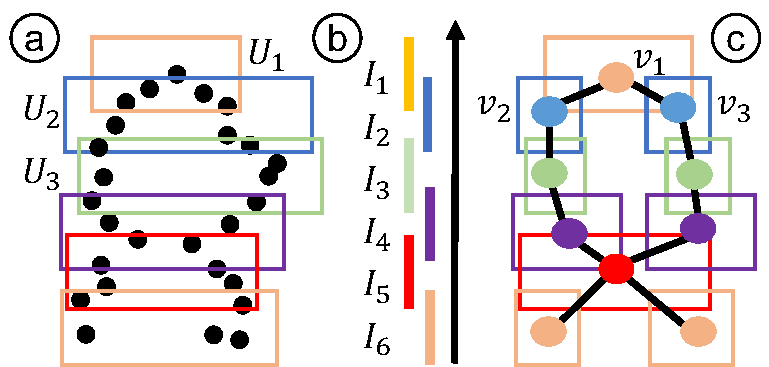
\includegraphics[width=\linewidth]{figures/toytda2.pdf}
    \caption{
      {\bf Toy Example of Mapper.} For a point cloud $\X$ (a), we define a lens function \textit{$f:\X\to\R$} (b), and the induced covering defines a Mapper graph where nodes represent clusters and edges represent related clusters (c). \label{fig:toyMapper}    }
\vspace{-.2in}
\end{wrapfigure}


After obtaining the nodes, we define the edges based on the intersections of the clusters. Note that as $I_k\cap I_{k+1}\neq \emptyset$, clusters in subsequent levels might have nontrivial intersections. Then, if the clusters $C_i\cap C_j\neq \emptyset$, we add an edge between the corresponding nodes $v_i$ and $v_j$. i.e., $\E=\{e_{ij}\mid C_i\cap C_j\neq \emptyset\}$ where $e_{ij}$ represents the edge between the nodes $v_i$ and $v_j$. It is also possible to define a weighted graph with weights $\omega_{ij}=\#(C_i\cap C_j)$, the count of the points in the intersection. In this case, the weights reflect the strength of the interaction between the corresponding clusters, indicating how many data points are included in the overlapped area. The final Mapper graph gives a rough summary/sketch of the whole point cloud. 

The Mapper graph not only helps in identifying data clusters but also enables the selection of data points that are similar to a given subset by leveraging its structure~\cite{bayir2022topological}. In this context, nodes that are closer together on the Mapper graph tend to contain more similar data points. This aspect of cluster similarity based on their proximity in the Mapper graph is an area that remains largely understudied and offers significant potential for further exploration. The Mapper graph computations have been detailed in \Cref{alg:mapper}. In~\Cref{sec:mapper-app}, we outline the utilization of Mapper in a real-life application, i.e., cancer genotyping from RNA sequencing.



\paragraph*{Common Filter Functions for Mapper.} While we explain the Mapper algorithm for single-valued filter functions to keep the exposition simpler, in practice it is very common to use multivariate filter functions $F:\X\to \R^2$. One of the most common filter functions used in applications is the \textit{Stochastic Neighborhood Embedding (t-SNE)}~\cite{hinton2002stochastic}, and a variant of this, called \textit{Neighborhood Lens}~\cite{gabrielsson2019exposition}. 

Similarly, it is common to use other dimension reduction techniques as filter map $F:\X\to \R^2$, e.g., Isomap, PCA, or UMAP~\cite{rather2022umap}. Then, for an open covering $\I=\{I_{ij}\}$ of $F(\X)$ in $\R^2$, one can repeat the process of $U_{ij}=F^{-1}(I_{ij})$, and assign a node $w$ for each cluster in $U_{ij}$. Again, assign an edge between the nodes when the corresponding clusters have nontrivial intersections. Note that if the domain of the data offers good filter functions $f,g:\X\to\R$,  one can also utilize multivariate filter functions $F(x)=(f(x),g(x))\in\R^2$ by combining both functions in the process. 


\subsubsection{Hyperparameters for Mapper} \label{sec:mapperParams}
For a point cloud $\X$, four main parameter choices must be made to obtain its Mapper graph. 

%The methods for selecting these parameters are often considered trade secrets and not shared in public documents. In our research, we have employed grid search~\cite{shamsi2024graphpulse, bayir2022topological} or back-testing in temporal settings~\cite{bitcoinheist2020} to determine the optimal parameters. While we briefly share our findings below in the hope they will be helpful, it’s important to note that the choice of parameters depends on the specific test case and should be optimized accordingly.


\begin{enumerate}
    \item \textit{The lens function.} If available, the lens function can be derived directly from the data domain, which in turn greatly enhances the interpretability of the model. In practice, when appropriate lens functions are not readily available from the data domain, dimensionality reduction techniques like t-SNE, UMAP, or PCA are commonly used to create lenses \( f: \mathcal{X} \to \mathbb{R}^2 \). 
    \item \textit{Clustering method.} For each subset $f^{-1}(I_k)$, the clustering method determines the nodes of the Mapper graph. The most common methods employed are DBSCAN and k-means, with their hyperparameters controlling the granularity of the resulting clusters.
    For k-means, it is common to use $<10$ for clusters (e.g., see~\cite[Figure 10]{shamsi2024graphpulse}).
    
    \item {\em Resolution and Overlap.} The resolution and overlap are the parameters for the covering $\{I_k\}_1^n$ of $f(\X)\subset \R$, i.e., $\bigcup_{k=1}^n I_k\supset f(\X)$. 
    The {\em resolution}, $n$, is the number of bins (intervals) $\{I_k\}$ to cover $f(\X)$. The {\em overlap} is the percentage of overlaps of these intervals, i.e. $\frac{|I_k\cap I_{k+1}|}{|I_k|}$.  Note that increasing the resolution gives a finer summary by increasing the number of nodes in the Mapper network and making the clusters smaller (See~\Cref{fig:mapper-bin}). On the other hand, increasing overlap adds more relation (edges) between the nodes (clusters).  In \Cref{fig:toyMapper}, the resolution is 6, and the overlap is the fixed intersection amount (e.g., 20\%) between the intervals $I_k$ and $I_{k+1}$. Typically, it is common to use $10\%-30\%$ overlap and 10-20 intervals (e.g., Figure 10 of GraphPulse~\cite{shamsi2024graphpulse}).
\end{enumerate}

 
 

\begin{algorithm}
\caption{Mapper Algorithm}
\label{alg:mapper}
\begin{algorithmic}[1]
\State \textbf{Input:} DataSet $\X$, Filter function $f: \X \to \mathbb{R}$, $\I = \{I_k\}$ covering of $f(\X)$ for a given resolution and overlap.
 
\State \textbf{Output:} Graph $\G$ (nodes and edges)
\State Initialize empty graph $\G$
\State Compute filter values: $f(\X)$
\For{each covering set $I_k$ in $\I$} \Comment{Defining nodes of $\G$}
    \State Compute preimage: $U_k = \{x \in \X \mid F(x) \in I_k\}$
    \State Cluster $U_k$ into clusters $\{C_i\}$
    \State Assign a node for each cluster, and get a set of nodes $\V_k$
    \State Add nodes in $\V_k$ to graph $\G$
\EndFor
\For{each pair of nodes $(v_i, v_j)$ in $\G$} \Comment{Defining edges of $\G$}
    \If{Clusters $C_i$ and $C_j$ have common points}
        \State Add edge $(v_i, v_j)$ to $\G$
    \EndIf
\EndFor
\State \textbf{Return} Graph $\G$
\end{algorithmic}
\end{algorithm}




\subsection{Mapper for Other Data Formats}  \label{sec:mapper-graph}
 

While the Mapper approach is most commonly applied to point clouds, it can be adapted for other data formats, such as graphs and images. For graphs, this adaptation can be seen as a form of graph coarsening/skeletonization, where the goal is to summarize clusters of nodes within the graph.

In~\cite{bodnar2021deep,hajij2018mog}, Bodnar et al. present a natural extension of the Mapper algorithm to the graph setting. Given a graph $\G=(\V,\E)$, we start with a filter function $f:\V\to\R$ and define a cover $\I = \{I_k\}_{k=1}^{n}$, where $\bigcup_k I_k \supset f(\X)$. The set $\V_k = f^{-1}(I_k)$ represents a subset of nodes, and $\G_k$ is the induced subgraph, i.e., $\G_k = (\V_k,\E_k)$ where $\E_k \subset \E$ are the edges connecting pairs of vertices in $\V_k$. Instead of clustering, we directly use the components (connected subgraphs) in $\G_k$ as the nodes of the Mapper graph.
Specifically, if $\G_{k_0} = \bigcup_{l=1}^{m_{k_0}} \G_{kl}$ has $m_{k_0}$ connected subgraphs, we define the node set $\C_k = \{c_{k_01}, \dots, c_{k_0m_{k_0}}\}$. For example, if $\G_k$ has five connected subgraphs, we define five nodes in the Mapper graph, each representing one connected subgraph in $\G_k$. Let $\W = \{w_1, w_2, \dots, w_M\}$ be the collection of all such nodes where $M = \sum_{k=1}^{n} m_k$. This defines the node set of the Mapper graph of $\G$. 

The edge set is defined similarly: If the subgraphs $\G_{kl}$ and $\G_{(k+1) l'}$ share a common node, then an edge is added between the corresponding nodes in $\W$. In summary, in the original construction, we replace the point cloud with the node set of $\G$, and the clustering algorithm is directly derived from the graph structure.  For this approach, one can utilize the common filtering functions $f:\V\to\R$ from persistent homology (e.g., degree, closeness, betweenness, eccentricity) or can use other popular functions from graph representation learning, e.g., eigenfunctions of graph Laplacian, pagerank~\cite{hajij2018mog}. 


 
Alternatively, if the graph \(\G = (\V, \E, \X)\) includes node attributes, a Mapper graph can be directly derived from the set of node attributes \(\X\). In particular, we treat the node attribute vectors \(\X = \{\X_i\}_1^n\) with \(\X_i \in \R^N\) as a point cloud \(\X \subset \R^N\) and apply the Mapper algorithm as before. This Mapper graph provides a visual summary of the node attribute space, independent of the graph's structure. In other words, the resulting Mapper graphs summarize the graph based on node attributes alone, without incorporating information about node neighborhoods in the original graph. An effective utilization of this approach can be found in~\cite{shamsi2024graphpulse}.


\begin{figure}[h!]
\centering
    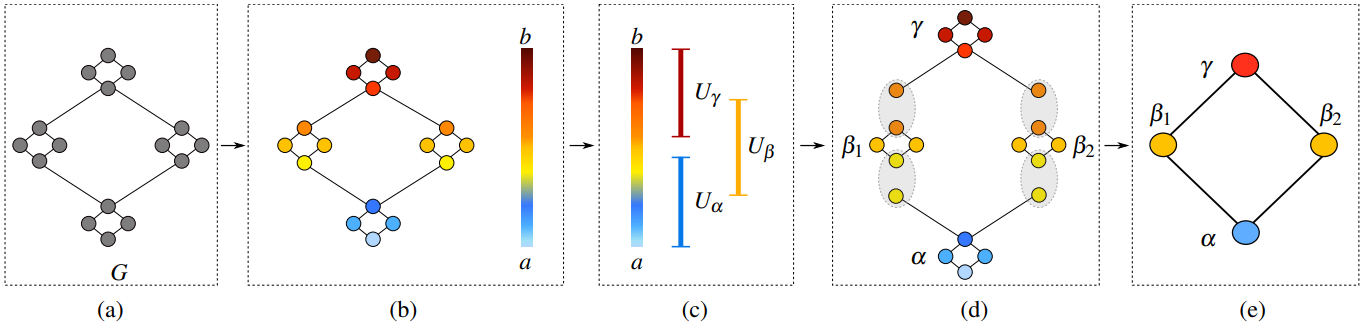
\includegraphics[width=\textwidth]{figures/mapper-for-graph.png}
    \caption{  {\bf Mapper for Graphs.} For a graph $\G$ (a), a filter function $f: \V \to \R$ (b), and the covering $\{U_\alpha, U_\beta, U_\gamma\}$ (c), we obtain the node clusters (connected subgraphs) (d), which define a Mapper network (e). The figure is adapted from~\cite{hajij2018mog}.\label{fig:mapper-graph}}
\end{figure}

The Mapper algorithm on images is analogous to its application in graphs, where clustering is derived from the original image~\cite{robles2017shape}. For a given \(r \times s\) image \(\X\), let \(f: \X \to \R\) represent the color values of the pixels. We define a cover \(\I = \{I_k\}_{k=1}^{n}\) such that \(\bigcup_k I_k \supset f(\X)\). A node is defined for each connected component in \(f^{-1}(\I_k)\), and an edge is created between nodes if the corresponding components have a nontrivial intersection. This Mapper graph summarizes the interaction between different color regions in \(\X\) as a graph.


\subsection{Computational Complexity of Mapper}
The computational complexity of TDA Mapper varies depending on the specific choices of filter functions, clustering algorithms, and dimensionality reduction techniques.  


The first step in TDA Mapper involves applying a filter function. If t-SNE is used as the filter, the computational complexity of the Barnes-Hut t-SNE variant is $\mathcal{O}(N \log N \cdot D)$~\cite{van2014accelerating}, where $N$ is the number of data points (e.g., for graphs, the number of nodes $|\mathcal{V}|$) and $D$ is the dimensionality of the data (e.g., for graphs, the number of node attributes). The complexity of t-SNE is largely driven by the computation of pairwise distances in a $D$-dimensional space, followed by optimizing the low-dimensional embedding. While dimensionality $D$ influences the time required for these computations, the overall complexity is typically dominated by the number of data points $N$.

After t-SNE, the data is covered by overlapping intervals, and clustering is performed within each interval. The complexity of this step depends on the clustering algorithm used. For example, if a clustering algorithm with complexity $\mathcal{O}(N^2)$ is used, this step may add significant computational cost. Finally, the Mapper complex is constructed by connecting clusters, which typically has a lower complexity, often $\mathcal{O}(N)$ to $\mathcal{O}(N \log N)$, depending on the number of clusters and the method used to connect them.

The overall computational complexity of TDA Mapper when using t-SNE is dominated by the complexity of t-SNE, which is $\mathcal{O}(N \log N \cdot D)$.  The subsequent steps in the Mapper pipeline add to this complexity, particularly the clustering step. When using $k$-means clustering, the complexity is typically $\mathcal{O}(k \cdot N \cdot D \cdot T)$, where $k$ is the number of clusters, $N$ is the number of data points, $D$ is the dimensionality of the data, and $T$ is the number of iterations. Therefore, the overall complexity can be expressed as $\mathcal{O}(N \log N \cdot D) + \mathcal{O}(k \cdot N \cdot D \cdot T)=\mathcal{O}(N \log N)$. 

\subsection{Software Libraries for Mapper} \label{sec:mapper-software}

Several software libraries provide tools for constructing and analyzing Mapper (see \Cref{tab:mapper-libraries}). Among these, Kepler-Mapper is a popular choice for Python users, particularly within the Scikit-TDA ecosystem, offering HTML outputs that are ideal for creating shareable, interactive visualizations. This makes it a practical tool for users who need to present their findings to non-technical users. 

Giotto-TDA integrates well with the Python environment and offers parameter visualization capabilities, making it an excellent choice for those needing to iteratively refine their Mapper construction. Its interactive features are especially helpful for real-time exploration of the impact of different filter functions and covering parameters.

For users prioritizing performance over interactivity, tda-mapper-python offers a faster computation engine, making it well-suited for large datasets or scenarios where rapid iteration is necessary. However, the lack of interactive features means that users will need to rely on external tools for visual exploration.

TDAmapper in R is an excellent choice for users already embedded in the R ecosystem. It’s a robust standalone solution that is particularly useful for those who prefer the extensive statistical and data manipulation capabilities available in R. However, the lack of interactivity might require additional effort for visualization and exploration.

Finally, Mapper Interactive is designed for those who value hands-on engagement with the data. It offers a highly interactive Python-based environment, making it ideal for exploratory data analysis where immediate feedback and manipulation of the Mapper graph are crucial.

In practice, the choice of library typically depends on the specific requirements of your project, such as whether you prioritize interactivity, computational speed, or seamless integration with other tools in your data analysis workflow. For example, Kepler-Mapper and Giotto-TDA are ideal for exploratory analysis and visualization, while tda-mapper-python and TDAmapper are more suitable for handling large-scale computations and integrating with ecosystems like Python and R, respectively.

 
\begin{table}[t]
\caption{Summary of TDA Mapper Libraries. \label{tab:mapper-libraries}}
\centering
\resizebox{1.\linewidth}{!}{
\begin{tabular}{l c  l c l}
\toprule
\textbf{Library Name}      & \textbf{Lang.}  & \textbf{Notable Feature}     &     \textbf{Interactive}     & \textbf{Code URL}                                 \\  \midrule 
\textbf{Kepler-Mapper~\cite{KeplerMapper_JOSS}}      & Python              & HTML output  &  \checkmark  & \small{\url{https://github.com/scikit-tda/kepler-mapper} (Scikit-TDA)}        \\  
\textbf{Giotto-tda~\cite{giottotda}}        & Python           & Parameter visuals    & \checkmark & \small{\url{https://github.com/giotto-ai/giotto-tda} }       \\   
\textbf{tda-mapper-python~\cite{simiMapper}} & Python             & Fast computation                          &     $\times$        & \small{\url{https://github.com/lucasimi/tda-mapper-python}} \\  
\textbf{TDAmapper}~\cite{singh2007topological}        & R                           & Standalone                          &           $\times$ & \small{\url{https://github.com/paultpearson/TDAmapper}}     \\  
\textbf{Mapper Interactive~\cite{zhou2021mapper}}         & Python                           & Interactive                          &           $\checkmark$ & \small{\url{https://github.com/MapperInteractive/MapperInteractive}}     \\  
%\textbf{Scikit-TDA} & Python& Wide Coverage & $\times$ &\small{\url{https://github.com/scikit-tda/scikit-tda}} \\
\bottomrule
\end{tabular}}
\end{table}

 
